\section{Novel contributions}\label{sec:novel-contributions}
 \todo{tengo qui o sposto nel cap 4?}

\subsection{Theory} \label{subsec:theory}
\todo{la discussione con l'esperto ci da' belief revision dei dati}
\todo{counterfactual explanations}
\todo{magari togliere theory e mettere tutto assieme}

\subsubsection{Selection based on entropy}
\todo{utilizzo entropia}

\subsection{Algorithms} \label{subsec:algorithms}
An important part of my work was developing the algorithms needed to adapt the ideas presented in the paper \enquote{Explaining the Most Probable Explanation} by \cite{Butz2018} and \enquote{A Progressive Explanation of Inference in \enquote{Hybrid} Bayesian} by \cite{Kyrimi2016}.
From the former, the construction of the probability tree through a constructive dialogue with the domain expert, the building of counterfactual explanation branches, the automatic generation of the most probable probability tree from initial evidence.
From the latter, the generation of an \enquote{Inverse explanation}.
Finally, a simple procedure to output a natural language explanation was developed.

\subsubsection{\enquote{Pseudo-MPE}} \label{subsubsec:pseudo-mpe}
\todo{dove critico il fatto che non calcolano veramente l'MPE come dicevano? qui o in cap.4 on cap.2?}
The so-called \enquote{Pseudo-MPE} algorithm is inherently wrapped up with the concept of \textit{dialogue} and is central to the explanatory powers of the system being developed in this thesis.
The algorithm was developed as a way of implementing the \enquote{MPE branch} of the \enquote{Argumentative Probability Tree} hypothesised by \cite{Butz2018}.
It was termed \enquote{Pseudo-MPE} because there are no guarantees of it returning the MPE solution (see Subsec. \ref{subsec:bnupdating}), as noted by \cite{koller2007introduction} in their definition of the MAP problem.

At a lower level of detail, the algorithm may be broken into:
\begin{itemize}
	\item a dialogical part, that interfaces with the expert user through the use of natural language, menus and visualisations
	\item the part responsible for constructing the \enquote{MPE branch}
\end{itemize}
The former process was informed and shaped by the results obtained by the methods described in Subsec. \ref{subsec:explainability-validation} and, as such, presented substantial elements of novelty.

The latter process is, at its core, a greedy procedure that aims at selecting the \enquote{best} next $(state, value)$ tuple at each step, based on some measure of optimality and on the variables already in the evidence set.
In the actual implemented system the two parts are intertwined, given their close inter-dependence.

The \texttt{dialogue} procedure starts by asking the user to select a subset of variables and their relative values to add as initial evidence.
This initial evidence is used to radicate the MPE Branch.
It should be noted than in the description given by \cite{Butz2018}, the Argumentative Probability Tree is a real tree as each node is guaranteed to have at most one parent.
My application, on the other hand, constructs an \textit{Argumentative Probability Polytree} (see Subsec. \ref{subsec:polytrees}) because, as will better be described in Chap. \ref{chap:results}, it was seen early on that the users much preferred to be able to start from a set of initial evidences and not be limited to a single one.
The algorithm then proceeds to call the \texttt{next\_most\_probable\_states} subroutine that is tasked with returning an ordered list of $(state,value)$ pairs.
It does this by calculating the posterior distribution given evidence of all the states not already in the evidence, then calculating the efficiency (see \ref{subsec:normalised-entropy}) and the maximally probable symbol of each state's distribution and finally returning the $(state,value)$ tuples ordered according to their normalised entropy (most efficient/least entropic at the head).
The $(state,value)$ pair at the head of the list is proposed to the user who has the faculty to accept the system's evaluation or refuse it.
If the user accepts, the state is added to the evidence set and to the MPE Branch under construction.
Thus, the evidence set's cardinality increases by one each time a user accepts a proposal.
The updated evidence will be used to calculate the new list of $(state,value)$ pairs at the following round.
If the expert chooses to refuse, then she is iteratively presented with the remaining $(state,value)$ items, in order of decreasing efficiency. 
Once she accepts one of the explanations given by the system, the \texttt{generate\_alternative\_branch} subroutine is called to automatically generate a maximally probable MPE Branch, radicated in the newest $(state,value)$ node of the MPE Branch.
The proposal loop for alternative states runs until there are increasingly less probable elements in the list and exits with a partial solution if the user refuses all of them at a given step.
Thus, the Pseudo-MPE solution is constructed only if the user runs through all variables proposed, accepting each one at least once.

Three slightly different operational modes of the algorithm were implemented.
This was done for research purposes, in order to understand which of the three, if any or if a combination of their distinctive features, the expert users would find the most useful from a usability, comprensibility and explainability standpoint:
\begin{itemize}
  \item exhaustive: In the basic dialogue type, the set of variables under consideration monotonically decreases by one every time the user accepts one of the system's proposals and the dialogue terminates only when the user has accepted all variables at least once or refused all proposals at a given step.
	In the first case the user will have the Pseudo-MPE solution while in the second she will be left with a partial assignment to some of the variables not present in the initial evidence.
	The pseudocode is shown in Alg. \ref{alg:pseudo-mpe-exhaustive}.
  \item d-separated: In the second variant, the set of variables under considered at each step is dynamic and depends on the separation properties of the underlying Bayesian Network's DAG and the evidence set constructed by the user's choices.
  	Differently from the first type of dialogue, an additional \texttt{evidence\_d\_separation} subroutine is called before \texttt{next\_most\_probable\_states} to calculate the set of variables that are d-separated from the evidence set, up to that step of the dialogue.
  	\texttt{next\_most\_probable\_states} is then executed but the variables that the previous function found to be separated from the evidence, are removed from the returned list.
  	This way, variables that can have no effect given the current evidence are not proposed.
  	As the d-separation operation is not monotonic, adding new nodes to the evidence set can both increment or diminish the number of nodes that will be proposed at each step.
  	The user is shown an updated view of the independencies of the graph at each step; an example of such an output is shown in Fig. \ref{fig:pseudo-mpe-independencies_1} and \ref{fig:pseudo-mpe-independencies_2}.
  	The pseudocode is shown in Alg. \ref{alg:pseudo-mpe-independencies}.
  \item thresholded: The final variant of the algorithm prunes the set of variables using a different strategy from the previously presented one.
  	In this case, the $(state,value)$ pairs in the list returned by \texttt{next\_most\_probable\_states} are dropped automatically based on their probability.
  	Pairs whose probability is below a user-defined threshold or are \enquote{worse than random} (for ex. a $(state,value)$ tuple will be discarded if $state$ is binary and the probability of $value$ is lower than $0.5$) are removed and not proposed to the user. 
  	This thresholding strategy based on the probability of the tuples is paired with one where there is a user-defined threshold on the number of times that the expert can refuse a particular $(state,value)$. 
  	In the general dialogue, tuples can be proposed multiple times, with an ever lower probability, if the user has previously refused them; in the thresholded scheme a $(state,value)$ pair can only be proposed a maximum number of times before being permanently discarded.
\end{itemize}

The underlying Bayesian Network that represents the data set is learned and queried through the  \texttt{pomegranate} (see Subsec. \ref{subsec:libraries}), API but the great majority of all the code is completely custom-written.
This was necessary because \texttt{pomegranate}, while having a powerful backend, was found to be severely lacking in the breadth and flexibility of its API.
Many basic operations, such as the calculation of a joint distribution, were not available so the only way was to implement lower-level workarounds while still using \texttt{pomegranate} for the most basic operations, as the calculation of a posterior distribution.
In particular, \texttt{dialogue} is implemented with the only direct calls to the API being when learning the network and when calling \texttt{predict\_proba}, that queries the \texttt{BayesianNetwork} object to calculate the posterior distribution of the states given the current evidence.
D-separation, in the second variant of the algorithm, is calculated via the \texttt{evidence\_d\_separation} procedure that implements the pseudocode presented in Alg. \ref{alg:d-separation}.

\begin{algorithm}[htp!]
	\caption{Exhaustive pseudo-MPE algorithm}
	\label{alg:pseudo-mpe-exhaustive}
	\begin{algorithmic}[1]
		\State $evidence = $ user selected $(state,value)$ tuples
		\State $MPE\_polytree = $ MPE Polytree rooted in $evidence$
		\While{True} 
			\State $mpe\_states$ = \texttt{next\_most\_probable\_states($evidence$)}
			\If{$mpe\_states$ is not empty}
				\State $next\_state$ = head of $mpe\_states$ 
				\State propose $next\_state$ to user \Comment{the least entropic state}
				\If{the user refuses $next\_state$}
					\For{$alternative\_state$ in $mpe\_states \smallsetminus next\_state$}
						\State propose $alternative\_state$ to user \Comment{the next least entropic states}
						\If{the user accepts $alternative\_state$}
							\State call \texttt{generate\_alternative\_branch()} on $MPE\_polytree$ 
							\State add $alternative\_state$ to $MPE\_polytree$
							\State $evidence = evidence \cup alternative\_state$
						\Else
							\State continue
						\EndIf
					\EndFor
				\Else
					\State add $next\_state$ to $MPE\_polytree$
					\State $evidence = evidence \cup next\_state$
				\EndIf
			\Else 
				\State return
			\EndIf
		\EndWhile
	\end{algorithmic}
\end{algorithm} 

\begin{algorithm}[htp!]
	\caption{Independencies pseudo-MPE algorithm}
	\label{alg:pseudo-mpe-independencies}
	\begin{algorithmic}[1]
		\State $evidence = $ user selected $(state,value)$ tuples
		\State $MPE\_polytree = $ MPE Polytree rooted in $evidence$
		\While{True} 
			\State $separated = $ \texttt{evidence\_d\_separation($evidence$)} \Comment{based on evidence of previous step}
			\State $mpe\_states$ = \texttt{next\_most\_probable\_states($evidence$)}
			\State $mpe\_states = mpe\_states \smallsetminus separated$ 
			\If{$mpe\_states$ is not empty}
				\State $next\_state$ = head of $mpe\_states$ 
				\State propose $next\_state$ to user \Comment{the least entropic state}
				\If{the user refuses $next\_state$}
					\For{$alternative\_state$ in $mpe\_states \smallsetminus next\_state$}
						\State propose $alternative\_state$ to user \Comment{the next least entropic states}
						\If{the user accepts $alternative\_state$}
							\State call \texttt{generate\_alternative\_branch()} on $MPE\_polytree$ 
							\State add $alternative\_state$ to $MPE\_polytree$
							\State $evidence = evidence \cup alternative\_state$
						\Else
							\State continue \Comment{go to next proposal}
						\EndIf
					\EndFor
				\Else
					\State add $next\_state$ to $MPE\_polytree$
					\State $evidence = evidence \cup next\_state$
				\EndIf
			\Else 
				\State return 
			\EndIf
		\EndWhile
	\end{algorithmic}
\end{algorithm} 

\begin{figure}[htbp]
\centerline{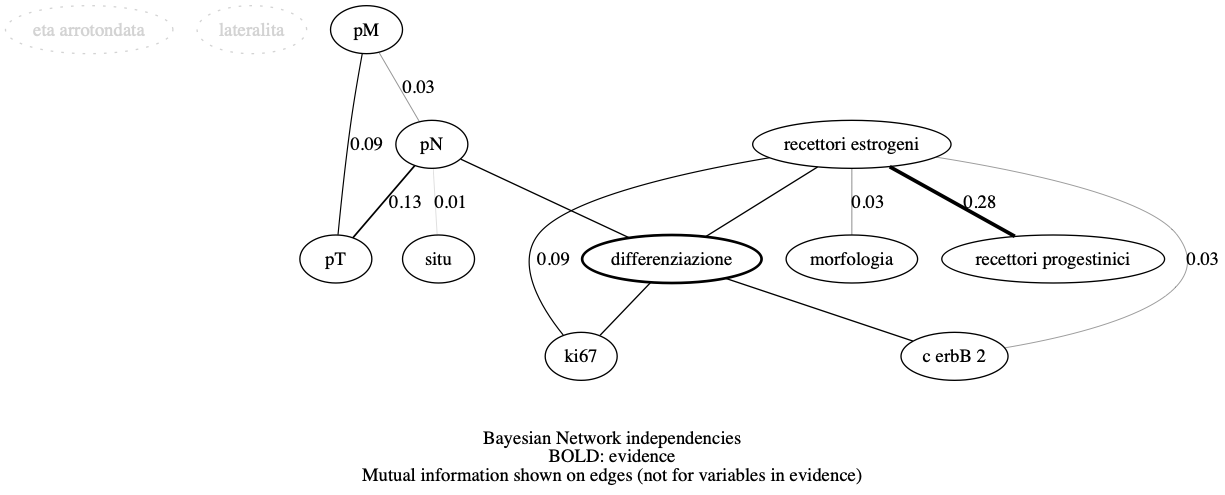
\includegraphics[width=\columnwidth]{methodology/images/example-d-separation-mpe_1}}
\caption{Example output during the first round of the d-separation-aware variant of \texttt{dialogue}.
	The variable \enquote{mut17q21} is the initial evidence.}
\label{fig:pseudo-mpe-independencies_1}
\end{figure}

\begin{figure}[htbp]
\centerline{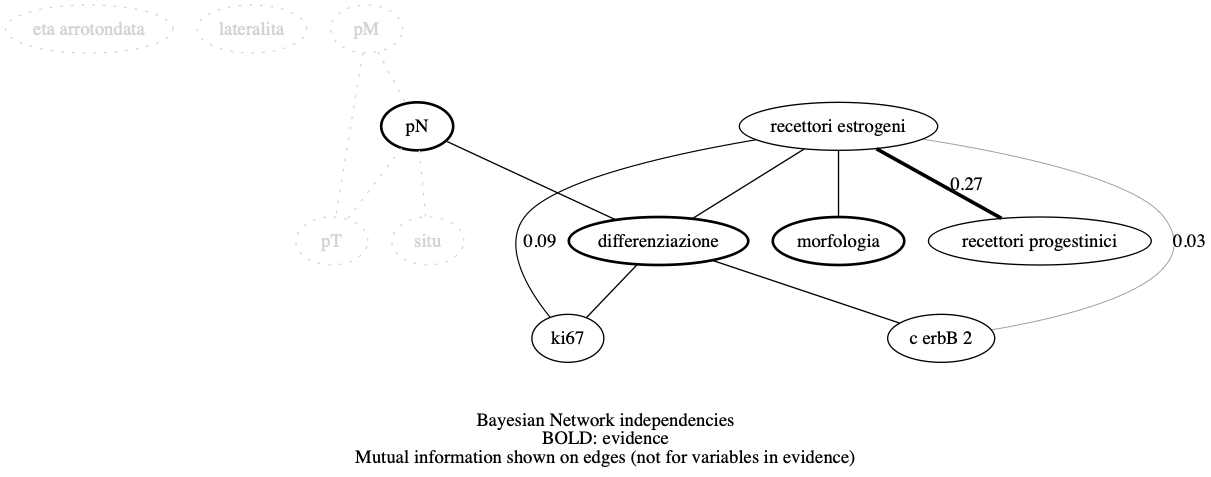
\includegraphics[width=\columnwidth]{methodology/images/example-d-separation-mpe_2}}
\caption{Example output during the second round of the d-separation-aware variant of \texttt{dialogue}.
	\enquote{morfologia} is added to the evidence set and this makes a large part of the network redundant.}
\label{fig:pseudo-mpe-independencies_2}
\end{figure}

\begin{algorithm}[htp!]
	\caption{Thresholded pseudo-MPE algorithm}
	\label{alg:pseudo-mpe-thresholded}
	\begin{algorithmic}[1]
		\State user selected $refuse\_bound$
		\State $refuse\_thresholds = \emptyset$
		\State $lower\_thresholds = \emptyset$
		\For{$v \in V$}
			\For{value $k$ of $v$}
				\State element $[v,k]=0$ in $refuse\_thresholds$
			\EndFor
			\State element $[v]=1 / |v|$ in $lower\_thresholds$ \Comment{refuse worse than random pairs}
		\EndFor
		\State $evidence = $ user selected $(state,value)$ tuples
		\State $MPE\_polytree = $ MPE Polytree rooted in $evidence$
		\State $mpe\_states$ = \texttt{next\_most\_probable\_states($evidence$)}
		\While{True} 
			\For{$s \in mpe\_states$}
				\If{probability of $s < lower\_thresholds[s] \wedge refuse\_thresholds[s] > refuse\_bound$}
					\State remove $s$ from $mpe\_states$ 
				\EndIf
			\EndFor		
			\If{$mpe\_states$ is not empty}
				\State $next\_state$ = head of $mpe\_states$ 
				\State propose $next\_state$ to user \Comment{the least entropic state}
				\If{the user refuses $next\_state$}
					\State increment $refuse\_thresholds[next\_state]$
					\For{$alternative\_state$ in $mpe\_states \smallsetminus next\_state$}
						\State propose $alternative\_state$ to user \Comment{the next least entropic states}
						\If{the user accepts $alternative\_state$}
							\State call \texttt{generate\_alternative\_branch()} on $MPE\_polytree$ 
							\State add $alternative\_state$ to $MPE\_polytree$
							\State $evidence = evidence \cup alternative\_state$
						\Else
							\State increment $refuse\_thresholds[alternative\_state]$
							\State continue
						\EndIf
					\EndFor
				\Else
					\State add $next\_state$ to $MPE\_polytree$
					\State $evidence = evidence \cup next\_state$
				\EndIf
			\Else 
				\State return
			\EndIf
		\EndWhile
	\end{algorithmic}
\end{algorithm} 

\subsubsection{Alternative Explanation Branches}
The function to generate alternative branches to the main MPE branch in the dialogue tree is called after the user refuses a $(state,value)$ in the dialogue and accepts one of the the alternatives.
The motivation is to present the user with a simple \enquote{what-if} analysis, replying to the question \enquote{Had I accepted the $(state,value)$ presented me by the system, what would have been the most probable configuration of the remaining $(state,value)$ pairs?}.
The question is answered by generating a maximally probable, alternative MPE sub-branch rooted in the last node in the main MPE branch that is under construction through the dialogue.

The alternative branch is generated by what is essentially an automated version of \texttt{dialogue} that always accepts the first suggestion returned by \texttt{next\_most\_probable\_states}.
Given that \texttt{dialogue} and \texttt{generate\_alternative\_branch} are essentially one and the same, the latter inherits the same pruning strategies as the former.
That is, \texttt{generate\_alternative\_branch} called during the exhaustive dialogue will generate a maximally likely assignment over all variables in $V \smallsetminus E$ while when invoked from one of the other two variant of the dialogue algorithm, it will apply their same pruning strategies.

The implementation of the MPE Polytree is based on the \texttt{NetworkX} python package (see Subsec. \ref{subsec:libraries}).
The creation of a chain of nodes is done by keeping a local pointer $alt\_node$ that refers to the last added node or set of nodes, if the node being added is the successor of multiple initial evidences. 

An example of the output shown to the user at each step of the dialogue is shown in Fig. \ref{fig:alternative-branch} while the pseudocode for the three variants are shown in Alg. \ref{alg:alternative-branch-echaustive}, \ref{alg:alternative-branch-independencies} and \ref{alg:alternative-branch-thresholded}.
Note that $alternative\_evidence$ is local to this algorithm and is separate from the $evidence$ used in the main \texttt{dialogue} procedure.

\begin{figure}[htbp]
\centerline{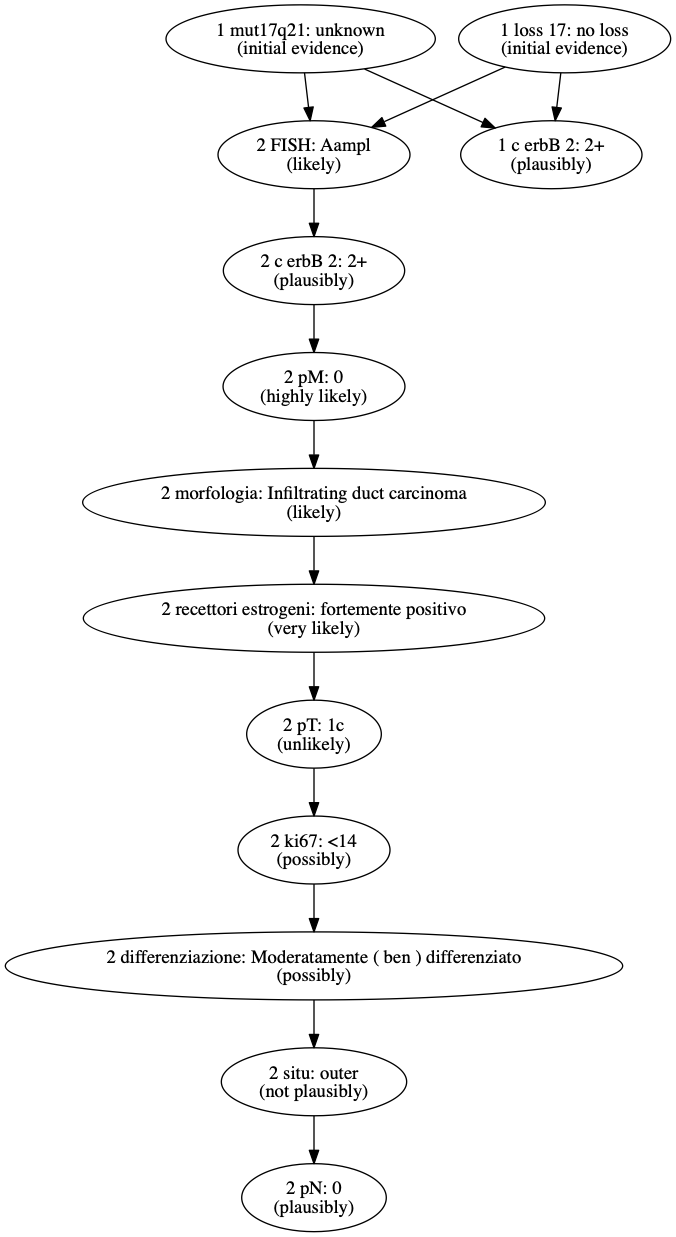
\includegraphics[scale=0.2]{methodology/images/alternative-explanation-tree-example}}
\caption{Example output during the d-separation-aware variant of \texttt{dialogue}.
	The tuple (\enquote{FISH},\enquote{Aampl}) was proposed but the expert refused it and accepted the alternative (\enquote{c erbB 2},\enquote{2+}).
	The main MPE Branch has ID 1 while the \enquote{what-if} one has ID 2.}
\label{fig:alternative-branch}
\end{figure}

\begin{algorithm}[htp!]
	\caption{Exhaustive alternative explanation branch algorithm}
	\label{alg:alternative-branch-echaustive}
	\begin{algorithmic}[1]
		\State $alternative\_evidence = evidence$ 
		\State $alt\_node = $ last node in the main MPE Polytree
		\State $branch\_id = branch\_id + 1$
		\While{True} 
			\State $mpe\_states$ = \texttt{next\_most\_probable\_states($alternative\_evidence$)}
			\If{$mpe\_states$ is empty}
				\State return
			\Else
				\State $next\_state$ = head of $mpe\_states$ 
				\State create $next\_state$ node, tag it with $branch\_id$ and make it son of $alt\_node$
				\State update $alt\_node$ node to be $next\_state$ node
				\State $alternative\_evidence = alternative\_evidence \cup next\_state$
			\EndIf
		\EndWhile
	\end{algorithmic}
\end{algorithm}

\begin{algorithm}[htp!]
	\caption{Independencies alternative explanation branch algorithm}
	\label{alg:alternative-branch-independencies}
	\begin{algorithmic}[1]
		\State $alternative\_evidence = evidence$ 
		\State $alt\_node = $ last node in the main MPE Polytree
		\State $branch\_id = branch\_id + 1$
		\While{True} 
			\State $separated = $ \texttt{evidence\_d\_separation($alternative\_evidence$)}
			\State $mpe\_states$ = \texttt{next\_most\_probable\_states($alternative\_evidence$)}
			\State $mpe\_states = mpe\_states \smallsetminus separated$ 
			\If{$mpe\_states$ is empty}
				\State return
			\Else
				\State $next\_state$ = head of $mpe\_states$ 
				\State create $next\_state$ node, tag it with $branch\_id$ and make it son of $alt\_node$
				\State update $alt\_node$ node to be $next\_state$ node
				\State $alternative\_evidence = alternative\_evidence \cup next\_state$
			\EndIf
		\EndWhile
	\end{algorithmic}
\end{algorithm} 

\begin{algorithm}[htp!]
	\caption{Thresholded alternative explanation branch algorithm}
	\label{alg:alternative-branch-thresholded}
	\begin{algorithmic}[1]
		\State $alternative\_evidence = evidence$ 
		\State $alt\_node = $ last node in the main MPE Polytree
		\State $branch\_id = branch\_id + 1$
		\While{True} 
			\For{$s \in mpe\_states$}
				\If{probability of $s < lower\_thresholds[s] \wedge refuse\_thresholds[s] > refuse\_bound$}
					\State remove $s$ from $mpe\_states$ 
				\EndIf
			\EndFor	
			\State $mpe\_states$ = \texttt{next\_most\_probable\_states($alternative\_evidence$)}
			\If{$mpe\_states$ is empty}
				\State return
			\Else
				\State $next\_state$ = head of $mpe\_states$ 
				\State create $next\_state$ node, tag it with $branch\_id$ and make it son of $alt\_node$
				\State update $alt\_node$ node to be $next\_state$ node
				\State $alternative\_evidence = alternative\_evidence \cup next\_state$
			\EndIf
		\EndWhile
	\end{algorithmic}
\end{algorithm} 

\todo{ancora da implementare true MPE}
\subsubsection{\enquote{Pseudo-MPE} from Random Evidence} \label{subsubsec: pseudo-mpe-random}
In order to compare the Pseudo-MPE output with the true MPE solution I implemented a simple algorithm that, starting from a random initial set of evidence, generates the relative pseudo-MPE and MPE solutions.
The random initial evidence set is constructed by randomly choosing a number in the interval $k = [ 1, |V| ]$, with $V$ the set of vertices in the BN, and then randomly selecting $k$ of the random variables in $V$ to yield the set of variables $E$.
The value of each variable is randomly chosen among the set of its values; as all variables are categorical, this can easily be done.

The implementation is based on the \texttt{NetworkX} python library (see Subsec. \ref{subsec:libraries}) package as what is being constructed is not a tree but a \textit{polytree} (see Subsec. \ref{subsec:polytrees}), as nodes may have multiple parents.
Note that $alternative\_evidence$ is considered separate from the main $evidence$ used in \texttt{dialogue}.

The pseudocode is shown in Alg. \ref{alg:pseudo-mpe-random-evidence} while an example output can be seen in Fig. \ref{fig:pseudo-mpe-random}.

\begin{algorithm}[htp!]
	\caption{Pseudo-MPE from random evidence algorithm}
	\label{alg:pseudo-mpe-random-evidence}
	\begin{algorithmic}[1]
		\State $evidence = \emptyset$
		\State generate random number $k \in [ 1, |V| ]$
		\State $S = $ choose $k$ variables from $V$
		\For{$s \in S$}
			\State choose random $v$ in the possible values of $e$ 
			\State $evidence = evidence \cup (s,v)$
		\EndFor
		\State $MPE\_polytree = $ MPE Polytree rooted in $evidence$
		\State $last\_node = evidence$
		\State $alternative\_evidence = evidence$ 
		\While{True} 
			\State $mpe\_states$ = \texttt{next\_most\_probable\_states($alternative\_evidence$)}
			\If{$mpe\_states$ is empty}
				\State return
			\Else
				\State $next\_state$ = head of $mpe\_states$ 
				\State create $next\_state$ node and make it son of $last\_node$
				\State update $alt\_node$ node to be $next\_state$ node
				\State $alternative\_evidence = alternative\_evidence \cup next\_state$
			\EndIf
		\EndWhile
	\end{algorithmic}
\end{algorithm}

\begin{figure}[htbp]
\centerline{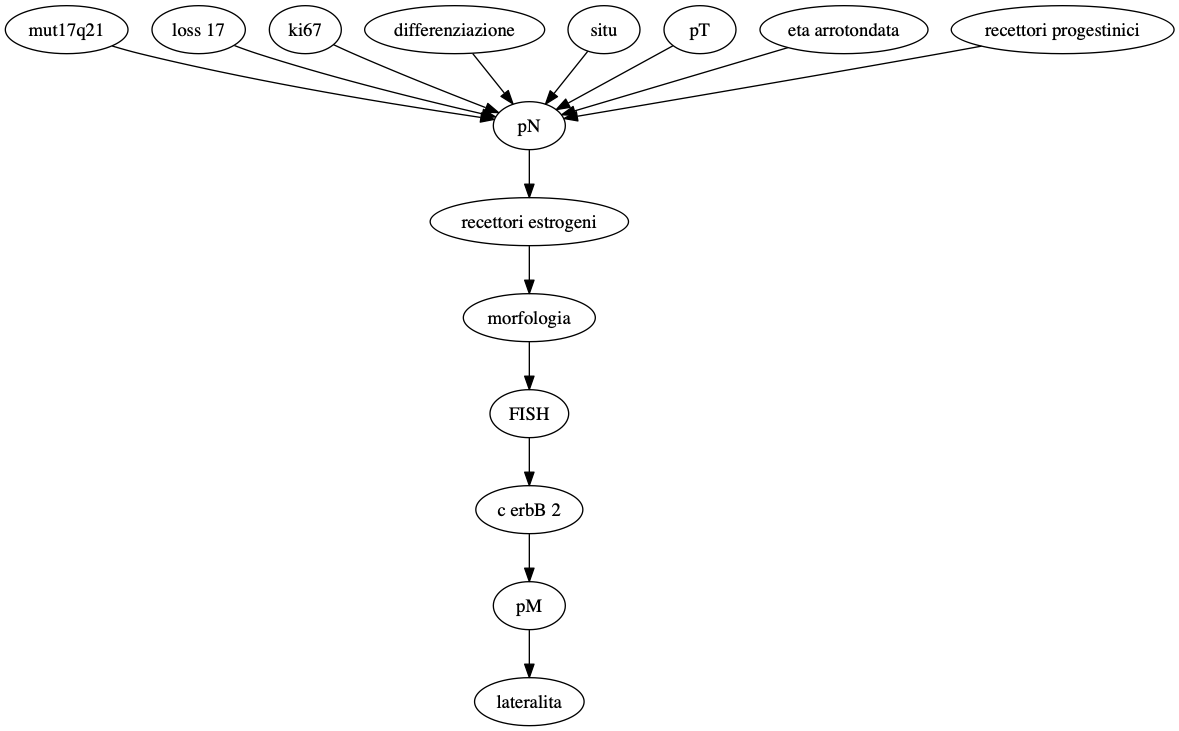
\includegraphics[width=\columnwidth]{methodology/images/pseudo-mpe-random-example}}
\caption{Example output of the Pseudo-MPE from random evidence algorithm.}
\label{fig:pseudo-mpe-random}
\end{figure}

\subsubsection{MPE algorithms comparison}
In order to compare the quality of the solution found using the simple Pseudo-MPE heuristic, I set up an experiment to compare it to the exact MPE solutions calculated with DAOOPT (see \ref{subsec:libraries}).
The user selects the number of iterations over which to average the results and at each iteration a Pseudo-MPE solution is generated using Alg. \ref{alg:pseudo-mpe-random-evidence}.
The same initial evidence is fed to DAOOPT using the \texttt{daoopt\_solver} interfacing procedure I wrote.

Returning to the example used while presenting DAOOPT in \ref{subsec:libraries}, given the \texttt{.uai} representing the BN and the \texttt{.uai.evid} random evidence:
\begin{verbatim}
 2
  4 1
  3 2
\end{verbatim}
DAOOPT would give the following output:
\begin{verbatim}
	--- Starting search ---
[0] u 3 4 -1.3581 5 2 1 2 2 1
[0] Cache statistics: . . . .

--------- Search done ---------
Problem name:  pomegranate
OR nodes:      3
AND nodes:     4
OR processed:  3
AND processed: 8
Leaf nodes:    2
Pruned nodes:  4
Deadend nodes: 1
Time elapsed:  0 seconds
Preprocessing: 0 seconds
-------------------------------
-1.3581 (0.0438433)

p 2 1 2
l 2 1 6
s -1.3581 5 2 1 2 2 1
\end{verbatim}
The end of the final line is the one of interest as it is the assignment of values to the variables that solves the MPE problem.
The \texttt{5 2 1 2 2 1} string is to be interpreted as meaning:
\begin{itemize}
  \item there are 5 variables in the solution
  \item the variable indexed by 0 (in the ordering given in the preable of the \texttt{.uai}) is assigned its second value (the ordering is inferred by the CPTs defined in the \texttt{.uai}) in the MPE solution
  \item variable 1 is assigned its first value
  \item variable 2 is assigned its second value
  \item variable 3 is assigned its second value
  \item variable 4 is assigned its first value
\end{itemize}
Variables 3 and 4 are constrained to assume the value specified in the input \texttt{.uai.evid}; in this case 1 and 2, respectively.

At each iteration corresponds a random evidence; the solutions given by the Pseudo-MPE and by DAOOPT are scored against each other using Hamming (Subsec. \ref{subsec:hamming-distance}) and Jaccard (Subsec. \ref{subsec:jaccard-distance}) distances on the vectors representing the returned assignments.
The sequence of distances is then averaged over the iterations to return the two averaged distances between the Pseudo-MPE and DAOOPT solutions to the MPE problem.

The implementation of the algorithm had to deal with the fact that DAOOPT failed on certain configurations of input evidence.
The reason for this is unknown so my workaround was to discard any iterations where DAOOPT had failed and retry them with another random set of evidences.
The pseudocode for the algorithm is shown in Alg. \ref{alg:mpe-comparison}.

\begin{algorithm}[htp!]
	\caption{MPE comparison algorithm}
	\label{alg:mpe-comparison}
	\begin{algorithmic}[1]
		\State user defined number of $iterations$
		\State initialise empty $results$ list
		\While{$i < iterations$}
			\State generate random number $k \in [ 1, |V| ]$
			\State $S = $ choose $k$ variables from $V$
			\For{$s \in S$}
				\State choose random $v$ in the possible values of $e$ 
				\State $evidence = evidence \cup (s,v)$
			\EndFor
			\State $pseudo\_mpe = $ \texttt{generate\_pseudo\_mpe($evidence$)}
			\State $model\_uai=$\texttt{export\_model\_to\_uai()}
			\State $evidence\_uai=$\texttt{export\_evidence\_to\_uai()}
			\State $daoopt\_mpe = $ \texttt{daoopt\_solver($model\_uai$, $evidence\_uai$)}
			\If{$daoopt\_mpe$ == -1} \Comment{DAOOPT has failed to calculate a solution}
				\State cancel $pseudo\_mpe$
				\State continue
			\EndIf
			\State compute $d_H(pseudo\_mpe,daoopt\_mpe)$, $d_J(pseudo\_mpe,daoopt\_mpe)$ and store in $iter\_result$
			\State append $iter\_result$ to $results$
			\State $i+=1$
		\EndWhile
		\State compute average in $results$ for $d_H$ and $d_J$
	\end{algorithmic}
\end{algorithm}

\subsubsection{Inverse Explanation}
\todo{da fare e trovare nome migliore}

\subsubsection{Natural Language Explanation}
\todo{da fare e magari pensare anche a visual explanations?}
The probability of each proposed tuple is quantified in natural language based on the probability of the most probable value within the variable.
These are shown in Tab. \ref{tab:naturallanguageprobabilities}.

\begin{table*}[htbp]
\caption{Probability quantifiers in natural language}
\begin{tabularx}{\textwidth}{@{} X X @{}}
\toprule 
Probability range & Natural language quantifier \\
\midrule 
(0, 0.2) &  "highly unlikely" \\
(0.2, 0.3) & "very unlikely" \\
(0.3, 0.4) & "unlikely" \\
(0.4, 0.5) & "not plausibly" \\
(0.5, 0.6) & "plausibly" \\
(0.6, 0.7) & "possibly" \\
(0.7, 0.8) & "likely" \\
(0.8, 0.9) & "very likely" \\
(0.9, 1) &  "highly likely" \\
(1) &  "certain" \\
\bottomrule
\end{tabularx}
\label{tab:naturallanguageprobabilities}
\end{table*}


\subsubsection{Pairwise Correlations}
An interesting addition, in terms of both explainability and theory, is an algorithm to measure and graphically display the interrelatedness between pairs of variables.
This is achieved by calculating the \textit{conditional mutual information} \todo{AA: e' giusto così?} between each pair of parent $\rightarrow$ child variables.
The definition of mutual information presented in Subsec. \ref{subsec:mutualinformation} is extended to account for the current state of the model i.e. the set of observed variables.
What we are calculating is:
\begin{equation}
	I(X,Y|E=e) = \sum_{x \in \mathcal{X}} \sum_{y \in \mathcal{Y}} p_{XY}(x,y|E=e) \log \left( \frac{p_{XY}(x, y|E=e)}{p_{X}(x|E=e) p_{Y}(y|E=e)} \right)
\end{equation}
This is not done if the parent variable, in the $X \rightarrow Y$ tuple under consideration, is in the evidence set; this is because observing a variable in a BN conceptually corresponds to disconnecting it from its children.

The implementation takes advantage of pgmpy's (\cite{pgmpy}) inference capabilities. 
To do this, I wrote a function to convert a pomegranate-based BN to an equivalent pgmpy-based one.
The queries to the model are done using the variable Elimination algorithm, that is more than suitable for a small BN.
The marginals for $X$ and $Y$ are calculated directly from the joint distributions, by marginalising the joint over one and then the other.
The function exits with $-1$ if the parent variable is in the evidence set.
As the mutual information $I(X,Y) \in [0,1]$ this signals to the calling function to treat this couple $X,Y$ differently.

The pseudocode for the algorithm is shown in Alg. \ref{alg:mutual-information}.

\begin{algorithm}[htp!]
	\caption{Mutual information algorithm}
	\label{alg:mutual-information}
	\begin{algorithmic}[1]
		\State $X$ parent variable in the BN DAG
		\State $Y$ child variable in the BN DAG
		\State $E$ set of current evidence in the BN
		\If{$X \in E$}
			\State return -1
		\EndIf
		\State $joint=p_{XY}(X, Y|E=e)$
		\State $Y\_marginal=$ marginalise $joint$ over $X$
		\State $X\_marginal=$ marginalise $joint$ over $Y$
		\State $mutual\_information = 0$
		\For{y in $Y\_marginal$}
			\For{x in $X\_marginal$}
				\State $j=$entry in $joint$ corresponding to $y$ and $x$
				\If{$j$ is $0$}
					\State $mutual\_information += 0$
				\Else
					\State $mutual\_information = j * log( j / ( y * x ) )$
				\EndIf
			\EndFor
		\EndFor
		\State return $mutual\_information$
	\end{algorithmic}
\end{algorithm}